\setcounter{section}{5}
\phantomsection
\section*{3. Data, Empirical Strategy and Results}
\addcontentsline{toc}{section}{3. Data, Empirical Strategy and Results}

This section describes the data sources, the construction of the analytical sample, and the empirical strategy, while also presenting the main descriptive patterns and empirical results. The dataset consists of European scholars and includes family relationships, academic careers, multiple measures of productivity and recognition, biographical traits, and regional inheritance systems. The empirical approach takes advantage of within-family variation between brothers to estimate birth-order effects controlling for unobserved family-level characteristics.

\phantomsection
\subsection*{3.1 Data Sources, Sample Construction and Descriptive Evidence}
\addcontentsline{toc}{subsection}{3.1 Data Sources, Sample Construction and Descriptive Evidence}

The dataset is constructed using the Repertorium Eruditorum Totius Europae (RETE) database, a secondary prosopographical source that provides biographical information on European scholars and is based on a wide range of historical materials \citep{curtis2026academic}. At the individual level, RETE includes information on year of birth and death, place of birth, and detailed records of academic activities and careers.

This secondary source is complemented with information drawn directly from primary historical sources, including published biographical repertories of university professors and academic elites. These repertories provide individual entries and often contain information on family relationships, such as fathers and siblings, which are used to identify and reconstruct family links between individuals.

When direct information on brothers in the secondary source or in a biographical dictionary is available, we use it. Second, we construct additional brother pairs by locating fathers with multiple sons in the academic records. For each father with at least two sons, all possible pairs of brothers are created.

Brother pairs are treated as unordered pairs and duplicates are removed. Pairs in which both siblings refer to the same individual are excluded. Birth order is determined using their birth year. A pair is classified as \emph{rankable} if the birth year is available for both brothers and the recorded birth years differ across siblings, allowing the unambiguous identification of the older and younger brother. Pairs are classified as \emph{unrankable} when the birth year is missing for at least one sibling or when both brothers share the same recorded birth year, making birth order impossible to establish with certainty. These observations are excluded from the birth-order regressions because the identification of older and younger siblings would otherwise require arbitrary assignment.

The final analytical sample used in the regression analysis consists of 645 rankable pairs of brothers for which birth order can be identified. Unrankable pairs are preserved for descriptive purposes and for analyzing how the composition and data quality of the sample evolve over time, although they are excluded from the empirical birth-order analysis. Appendix Figure~\ref{fig:rankable_unrankable} presents the distribution of rankable and unrankable brother pairs across centuries. The figure shows that observations with identifiable birth order are available throughout the full historical period covered by the dataset.

Appendix Table~\ref{tab:rankable_compare} compares rankable and unrankable brother pairs. Rankable pairs display substantially higher scholarly visibility and lower rates of zero productivity, suggesting that observations with identifiable birth order are positively selected toward scholars with richer historical records.

In total, approximately 71\% of identified brother pairs are rankable, while the remaining observations are classified as unrankable due to missing or identical year of birth.

The summary statistics for the analytical sample are reported in Table~\ref{tab:descriptives}. Information on the timing of entry into academia is proxied using the first recorded academic activity for each individual. Appendix Figure~\ref{fig:age_entry} presents the distribution of age at entry into academia. While most scholars enter in early adulthood, a small number of observations display very early entry ages, which may reflect early university enrollment or measurement imprecision in historical records.

\begin{table}[H]
\centering
\caption{Descriptive Statistics}
\label{tab:descriptives}

\begin{tablebody}
\begin{tabular}{l c}
\toprule
\textbf{Statistic} & \textbf{Value} \\
\midrule
Number of brother pairs & 645 \\
Mean entry age in academia & 32.93 \\
Mean age gap (years) & 7.22 \\
Father in academia (share) & 38.8\% \\
Titles (older brother) & 11.89 \\
Titles (younger brother) & 9.79 \\
Older brother more productive (share) & 41.6\% \\
Younger brother more productive (share) & 31.3\% \\
Share of individuals with no titles & 40.2\% \\
Share of pairs with no titles & 25.4\% \\
\bottomrule
\end{tabular}
\end{tablebody}

\vspace{4pt}
\begin{minipage}{\textwidth}
\footnotesize
\textit{Notes:} Descriptive statistics for the sample of rankable brother pairs, i.e. pairs for which birth order can be identified, unless otherwise indicated. Scholarly productivity is measured using the number of titles recorded in VIAF. The mean entry age into academia is computed using all scholars with available information on birth year and first recorded academic activity. Shares are reported as percentages.
\end{minipage}

\end{table}
\FloatBarrier

There is considerable variation in age gaps between brothers, with an average of 7.2 years. The distribution of age gaps is presented in Appendix Figure~\ref{fig:age_gap}. The presence of large age differences highlights the importance of controlling for age gaps in the empirical analysis, in order to distinguish birth-order effects from cohort and life-cycle differences.

About 39\% of scholars in the sample had a father who was also active in academia. The sample is drawn from the same historical database used in \citet{DelacroixGoni2024}. We therefore control for paternal academic background in the empirical analysis.

Older brothers appear slightly more productive on average. The average number of titles associated with VIAF is 11.89 for older brothers and 9.79 for younger brothers. However, this difference does not imply that older brothers systematically outperform their siblings. Figure~\ref{fig:birthorder_pie} illustrates the distribution of within-family productivity comparisons: older brothers are more productive in 42\% of pairs, while younger brothers outperform their older siblings in about 31\% of cases, and productivity is equal in the remaining pairs. An additional important feature of the sample is the large share of scholars with no recorded titles: approximately 40\% of individuals and 25\% of brother pairs have zero observed titles.

\begin{figure}[H]
\centering
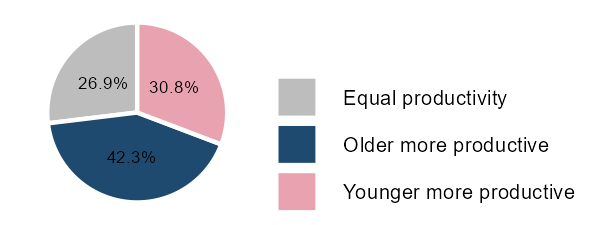
\includegraphics[width=0.65\textwidth]{figures/Pie_Productivity_BirthOrder.png}

\caption{Productivity comparison between older and younger brothers}
\label{fig:birthorder_pie}

\vspace{4pt}
\begin{minipage}{\textwidth}
\footnotesize
\textit{Notes:} The figure shows the distribution of within-family productivity comparisons between older and younger brothers. Shares indicate the proportion of brother pairs in which the older brother has more titles recorded in VIAF, the younger brother has more titles, or both brothers have the same number of titles.
\end{minipage}

\end{figure}
\FloatBarrier

This pattern reflects substantial heterogeneity in within-family productivity differences. While there is a modest average advantage for older brothers, productivity differences vary widely across families and are far from universal. This heterogeneity is particularly visible across historical periods, as shown in Appendix Figures~\ref{fig:productivity_period} and~\ref{fig:birthorder_period}. 

Additional descriptive statistics by historical period are presented in Appendix Table~\ref{tab:prepost16}. The table shows that scholars observed before the sixteenth century tend to exhibit higher average productivity levels and larger age gaps between siblings, although the earlier subsample is substantially smaller. 

While the dataset provides a rich and detailed perspective, it reflects a selected sample of scholars who left observable traces in historical records and may therefore over-represent individuals with higher visibility. In addition, bibliographic indicators such as VIAF title counts may partly reflect the long-run accumulation of editions, translations, republications, and archival preservation over time. Although the empirical analysis controls for historical periods, scholars from earlier centuries may have had more opportunity to accumulate observable bibliographic traces in historical records.

This heterogeneity can be illustrated with concrete examples from the dataset. In some cases, differences between siblings are relatively small. For instance, the Bernoulli brothers, well-known figures in the history of mathematics, display very similar levels of scholarly productivity, with Jacob Bernoulli having 63 titles recorded in VIAF and Johann Bernoulli 59. Their prominence in the scientific revolution makes them a natural benchmark for comparing within-family outcomes.

In other cases, however, productivity differences are substantially larger. The Thomasius brothers provide a contrasting example: Christian Thomasius is associated with 71 titles, whereas his younger brother Gottfried Thomasius has only 5. In this case, we did not select the pair of brothers for its historical prominence, but because it exhibits one of the largest productivity gaps observed in the data, making it particularly informative for illustrating the extent of within-family heterogeneity.

At the same time, many of the sibling pairs driving this heterogeneity are less visible in historical narratives. For example, August Ludwig Schott (1751–1787) and his younger brother Andreas Heinrich Schott (1758–1831) can be clearly ranked by age, and both exhibit measurable scholarly activity (with 4 and 6 recorded titles, respectively), yet neither individual has a significant presence in accessible sources. This kind of pair of brothers is identified through prosopographical data. Notably, both are linked to the same academic environment as their father, further illustrating how such patterns can only be uncovered through structured historical sources.

Taken together, these examples highlight the wide dispersion of within-family outcomes and reinforce the idea that birth-order advantages are not universal, but instead coexist with substantial heterogeneity across families.

Because scholarly productivity is highly skewed and rewards may follow a convex function of talent under superstar-type dynamics \citep{curtis2026academic}, the analysis uses the inverse hyperbolic sine transformation of titles to obtain a more concave measure of output differences. Figure~\ref{fig:titles_distribution} shows the resulting distribution of scholarly productivity for older and younger brothers. The two distributions largely overlap, although the distribution for older brothers is slightly shifted to the right, indicating a modest productivity advantage. The concentration of observations near zero reflects the highly skewed nature of historical scholarly output.

\begin{figure}[H]
\centering
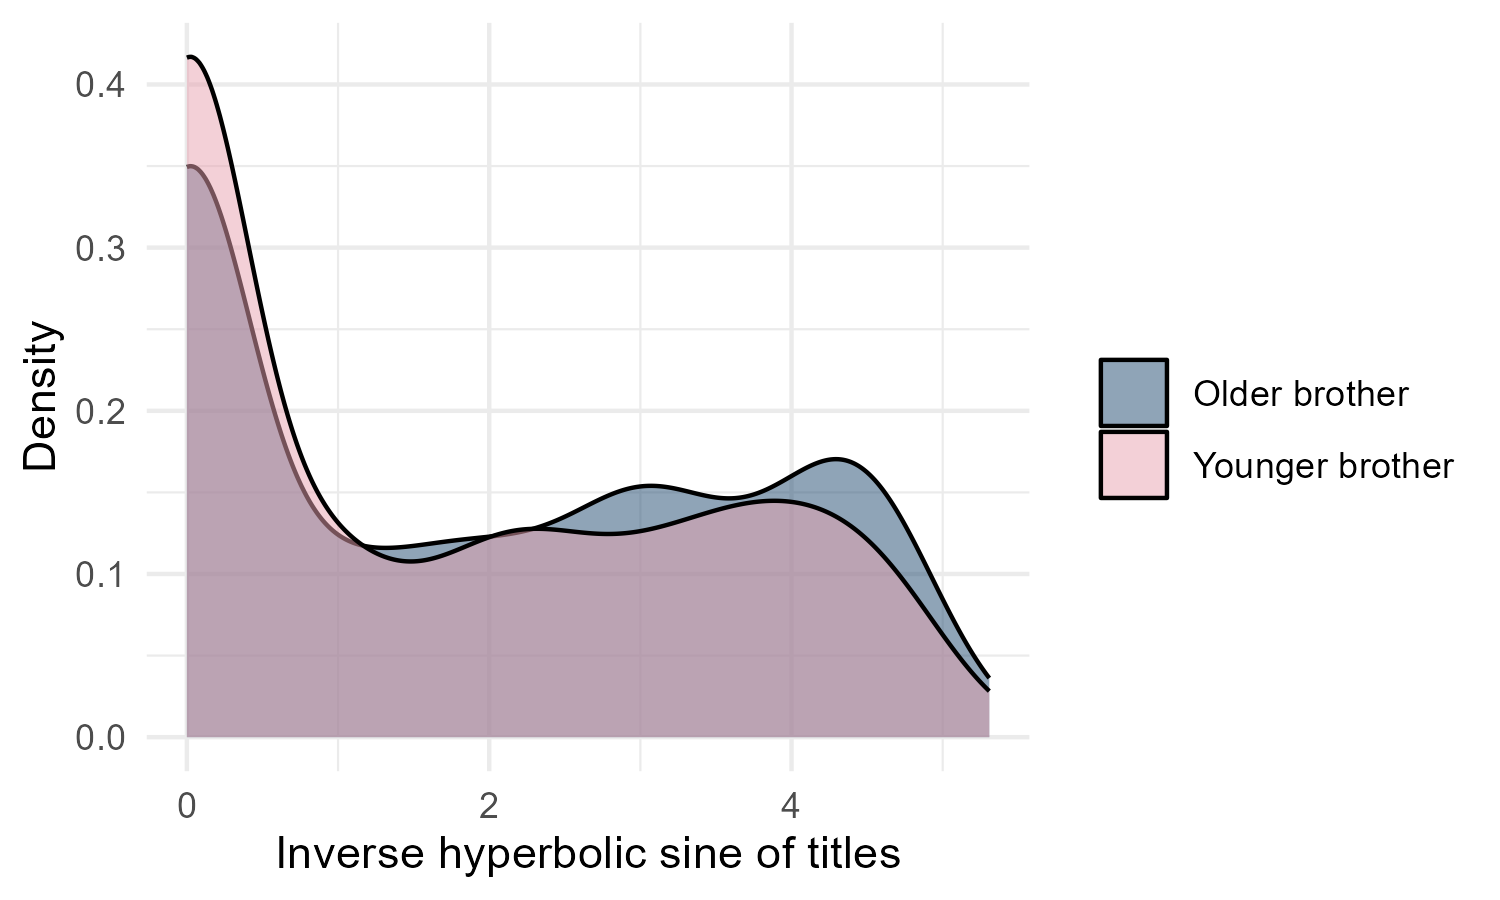
\includegraphics[width=0.65\textwidth]{figures/Plot_Productivity_Distribution.png}

\caption{Distribution of scholarly productivity by birth order}
\label{fig:titles_distribution}

\vspace{4pt}
\begin{minipage}{\textwidth}
\footnotesize
\textit{Notes:} The figure compares the distribution of scholarly productivity between older and younger brothers. Productivity is measured using the inverse hyperbolic sine transformation of the number of titles recorded in VIAF.
\end{minipage}

\end{figure}
\FloatBarrier

\phantomsection
\subsection*{3.2 Outcome Variables and Paired Comparisons}
\addcontentsline{toc}{subsection}{3.2 Outcome Variables and Paired Comparisons}

The primary outcomes of interest reflect academic productivity and recognition. Productivity is measured using bibliometric indicators derived from the Virtual International Authority File (VIAF), including the number of titles attributed to an individual, as well as the number of publishers, publication countries, coauthors, and works with ISBN identifiers.

Recognition is proxied using Wikipedia-based measures, including the length of articles and the number of languages in which an individual is represented. These measures capture visibility and perceived importance in the historical record, complementing bibliographic indicators of scholarly output, although they may not fully reflect underlying intellectual ability or informal scholarly contributions not recorded in historical sources.

Additional measures derived from Wikidata include the number of occupations associated with each scholar and the number of recorded academic affiliations. These variables aim to capture broader dimensions of scholarly activity and institutional involvement beyond bibliographic output \citep{curtis2026academic}.

As these variables are highly skewed with a large number of zero observations, the analysis uses the inverse hyperbolic sine transformation. Formally, this transformation is defined as: $\text{asinh}(x)=\ln(x+\sqrt{x^2+1})$.

The inverse transformation is given by: $\sinh(z)=(e^z-e^{-z})/2$. This allows changes in asinh units to be translated back into the original scale of titles.

This transformation behaves similarly to the logarithmic transformation for large values of $x$, while remaining well-defined at zero. Unlike a standard logarithmic specification, percentage interpretations of differences in asinh-transformed variables depend on the baseline level of the variable \citep{aihounton2021units}. To facilitate the interpretation of coefficients in asinh-transformed units, implied percentage differences are evaluated at representative productivity levels using:
\[
\%\Delta y
=
100 \times
\left(
\frac{
\sinh\left(
\operatorname{asinh}(y_0)+\beta
\right)
}{
y_0
}
-1
\right),
\]
where $y_0$ denotes the baseline productivity level and $\beta$ the estimated difference in asinh-transformed outcomes. This allows approximate percentage interpretations while accounting for the non-linear behavior of the transformation near zero.

To ensure that the results are not driven by the choice of functional form, additional robustness checks reported later in the paper replicate the main specifications using both logarithmic and level specifications of productivity differences.

By assigning outcomes independently to the older and younger brothers for rankable pairs, we conduct direct within-family comparisons. Table~\ref{tab:ttests} presents paired comparisons of older and younger brothers across all productivity and recognition measures.

Older brothers tend to perform slightly better than their younger siblings on several dimensions of scholarly productivity. On average, older brothers hold 2.10 more titles in VIAF than younger brothers, a difference that is statistically significant at conventional levels.

Evaluated at the mean productivity level of younger brothers ($y_0 = 9.79$ titles), the asinh difference of 0.245 implies an approximate productivity advantage of 27.5\% for older brothers. We used the formula presented previously to compute this percentage: $100 \times \left(\frac{\sinh\left(\operatorname{asinh}(9.79)+0.245\right)}{9.79}-1\right)\approx 27.5\%$.

Because the inverse hyperbolic sine transformation is non-linear near zero, this interpretation should be viewed as an approximation rather than as a constant semi-elasticity.

This pattern also appears when considering alternative measures of scholarly prominence. Older siblings tend to have longer Wikipedia pages, more language versions, more publishers, and more coauthors. They are also more likely to have at least one title recorded in VIAF, indicating a higher probability of entry into scholarly production.

However, the size of these differences varies across indicators and is not statistically significant for all outcomes. This suggests that while there is a consistent tendency for older brothers to outperform younger siblings, the magnitude of the effect remains moderate.

Appendix Table~\ref{tab:period_ttests} reports paired comparisons separately before and after the sixteenth century. The older-brother productivity advantage appears larger in the earlier subsample, although estimates for the pre-sixteenth-century period are based on a considerably smaller number of observations. In particular, the mean asinh productivity difference reaches 1.046 before the sixteenth century, compared with 0.202 in later periods.

Overall, the evidence from paired comparisons points to a modest but systematic older-brother advantage in scholarly productivity and visibility. At the same time, the heterogeneity observed across families indicates that birth order is only one of several factors shaping academic outcomes.

This finding is consistent with the literature on modern populations, which documents an older-brother advantage in educational attainment and long-run outcomes \citep{Black2005, Behrman1986}. However, the magnitude of the effect observed in this historical sample is relatively modest, in line with recent historical evidence suggesting weaker or more context-dependent birth-order effects \citep{ClarkCummins2024}.

\begin{table}[H]
\centering
\caption{Paired Differences Between Older and Younger Brothers}
\label{tab:ttests}

\begin{tablebody}
\begin{tabular}{l c c c c}
\toprule
\textbf{Measure} & \textbf{Mean Diff.} & \textbf{p-value} & \textbf{N} \\
\midrule
Titles (VIAF) & 2.096 & 0.0076 & 645 \\
Titles (VIAF, asinh) & 0.245 & 0.0007 & 645 \\
Longest Wikipedia page (chars) & 409.788 & 0.0453 & 645 \\
Longest Wikipedia page (asinh) & 0.182 & 0.0228 & 645 \\
Has at least one title & 0.056  & 0.0089 & 645 \\
Number of Wikipedia languages & 0.659 &  0.0215 & 645 \\
Publication countries (VIAF) & 0.372 &  0.0140 & 645 \\
Publishers (VIAF) & 0.667 & 0.0043 & 645 \\
Coauthors (VIAF) & 1.056 & 0.0001 & 645 \\
Publications with ISBN & 0.381 & 0.1158 & 645 \\
Publications before 1900 & 21.667  & 0.0013 & 645 \\
Publications after 1900 & 1.932  & 0.1904 & 645 \\
Academic affiliations (Wikidata) & 0.130  & 0.0626 & 645 \\
Number of occupations (Wikidata) & 0.171  & 0.0328 & 645 \\
Number of positions & -0.033  & 0.5849 & 645 \\
Longevity (years) & -0.180  & 0.8297 & 579 \\
\bottomrule
\end{tabular}
\end{tablebody}

\vspace{4pt}
\begin{minipage}{\textwidth}
\footnotesize
\textit{Notes:} Paired t-tests comparing older and younger brothers across productivity and recognition measures. Mean differences are calculated as older minus younger. Variables transformed using the inverse hyperbolic sine transformation are discussed in the main text.
\end{minipage}

\end{table}
\FloatBarrier

\phantomsection
\subsection*{3.3 Extensive and Intensive Margins of Productivity}
\addcontentsline{toc}{subsection}{3.3 Extensive and Intensive Margins of Productivity}

To better understand the mechanisms underlying birth-order differences in scholarly productivity, we decompose academic output into extensive and intensive margins. This distinction allows us to assess whether birth order primarily affects entry into scholarly activity or productivity conditional on participation.

The extensive margin captures whether a scholar has at least one publication recorded, while the intensive margin measures productivity conditional on having published. The extensive margin is estimated using a logit specification, whereas the intensive margin is estimated using OLS with an inverse hyperbolic sine transformation of titles. Both specifications control for age gaps between siblings and whether the father was active in academia, with standard errors clustered at the family level.

Table~\ref{tab:extensive_intensive} presents the regression results. The estimates show that older brothers are significantly more likely to have at least one publication recorded. The coefficient on the indicator for being the older sibling is positive and statistically significant, indicating that older siblings are significantly more likely to enter scholarly production. The estimated coefficient of 0.238 in the logit specification corresponds to an odds ratio of approximately $e^{0.238} \approx 1.27$, implying that older brothers have approximately 27\% higher odds of having at least one recorded publication than their younger siblings. In other words, holding age gap and family background constant, older brothers are substantially more likely to appear in the historical record with at least one identified publication.

Although the coefficient on the older-sibling indicator remains positive in the intensive-margin specification, it is statistically insignificant, suggesting that conditional productivity differences are limited once scholars enter academic production.

Taken together, these results indicate that birth-order effects operate primarily through the extensive margin. Older siblings are more likely to become active scholars, while conditional productivity differences remain limited. This pattern is consistent with theories of parental investment, which emphasize differential access to opportunities rather than performance among those who participate \citep{Becker1976, Hotz2015}. In historical contexts in which access to academic careers required substantial family investment and social connections, older siblings may have benefited from preferential allocation of resources, such as education or access to networks, increasing their likelihood of entering academia. Once these barriers are overcome, however, long-run productivity appears to depend more on individual ability and institutional opportunities than on birth order, although this interpretation relies on observed publication records and cannot capture unrecorded scholarly activity.

\begin{table}[H]
\centering
\caption{Extensive and Intensive Margins of Scholarly Productivity}
\label{tab:extensive_intensive}

\begin{tablebody}
\begin{tabular}{l c c}
\toprule
 & \textbf{Extensive (Logit)} & \textbf{Intensive (OLS)} \\
 & \textit{Pr(Title $>0$)} & \textit{Asinh titles} \\
\midrule

Constant
& 0.051 & 2.892*** \\
& (0.129) & (0.101) \\

Older sibling
& 0.238*** & 0.141 \\
& (0.091) & (0.089) \\

Age gap
& -0.002 & -0.013 \\
& (0.012) & (0.009) \\

Father in academia
& 0.654*** & 0.090 \\
& (0.176) & (0.112) \\

\midrule
Clustered SE (family) & Yes & Yes \\
\midrule
Observations & 1290 & 772 \\
R$^{2}$ &  & 0.008 \\
Adj. R$^{2}$ &  & 0.004 \\
\bottomrule
\end{tabular}
\end{tablebody}

\vspace{4pt}
\begin{minipage}{\textwidth}
\footnotesize
\textit{Notes:} Column (1) reports logit estimates for the probability of having at least one title recorded in VIAF. Column (2) reports OLS estimates conditional on positive titles using the inverse hyperbolic sine transformation of titles. Standard errors are clustered at the family level. \textit{Significance levels:} *** $p<0.01$, ** $p<0.05$, * $p<0.10$.
\end{minipage}

\end{table}
\FloatBarrier

\phantomsection
\subsection*{3.4 Institutional Environment and Inheritance Systems}
\addcontentsline{toc}{subsection}{3.4 Institutional Environment and Inheritance Systems}

To account for institutional variation across regions, the analysis incorporates information on inheritance systems following the classification developed by \cite{Todd1990}, with adaptations for France based on \cite{Gobbi2024}. Regions are categorized according to their predominant inheritance regime, distinguishing between egalitarian and non-egalitarian systems.

Inheritance regimes are assigned to scholars based on their birthplace using a geographic mapping at the NUTS3 level, although this regional assignment may mask within-region heterogeneity in actual family practices. For brother pairs with known birth order, the inheritance regime is associated with the birthplace of the older brother. Because the data only contain scholars observed in RETE, the older observed brother may not always coincide with the biological firstborn of the family, implying that the analysis captures birth-order differences among observed scholarly siblings rather than strict primogeniture status.

Figure~\ref{fig:todd_map} provides a geographic visualization of inheritance systems alongside the birthplaces of scholars in the dataset. Shaded areas represent Todd’s typology of inheritance regimes, while circles indicate the number of scholars born in each location.
Scholars in the dataset are distributed across a wide range of European regions, spanning diverse institutional environments. Among observations with classified inheritance systems, approximately 47\% correspond to non-egalitarian regimes and 30\% to egalitarian ones. A non-negligible share of observations remains unclassified because some regions cannot be matched precisely to Todd's typology. These proportions are reported in more detail in Appendix Table~\ref{tab:inheritance_composition}, which also shows that approximately 23\% of observations remain unclassified because some regions are not assigned to either egalitarian or non-egalitarian inheritance systems in Todd’s typology.

This variation across space provides the basis for examining whether inheritance institutions are associated with the within-family productivity differences.

To capture the temporal dimension of this variation, Figure~\ref{fig:inheritance_century} shows the share of brother pairs born in regions characterized by non-egalitarian inheritance systems by century.

Figure~\ref{fig:inheritance_century} indicates that non-egalitarian inheritance systems remain prevalent across the sample, although their relative importance varies over time. This spatial and temporal variation provides the empirical foundation for examining whether inheritance institutions are associated with within-family productivity differences across historical periods.

Importantly, Figure~\ref{fig:inheritance_century} also shows that non-egalitarian inheritance systems are almost absent in the thirteenth and fourteenth centuries of the sample. For this reason, some supplementary specifications reported in the Appendix distinguish between observations before and after the sixteenth century, in order to account for the limited variation in inheritance systems during the earlier centuries of the sample.

In principle, inheritance institutions may influence parental investment decisions. In non-egalitarian systems, such as primogeniture, family resources and opportunities may have been concentrated toward older sons, potentially reinforcing birth-order advantages. In contrast, egalitarian systems may distribute resources more evenly across siblings, reducing such differences.

\begin{figure}[H]
\centering
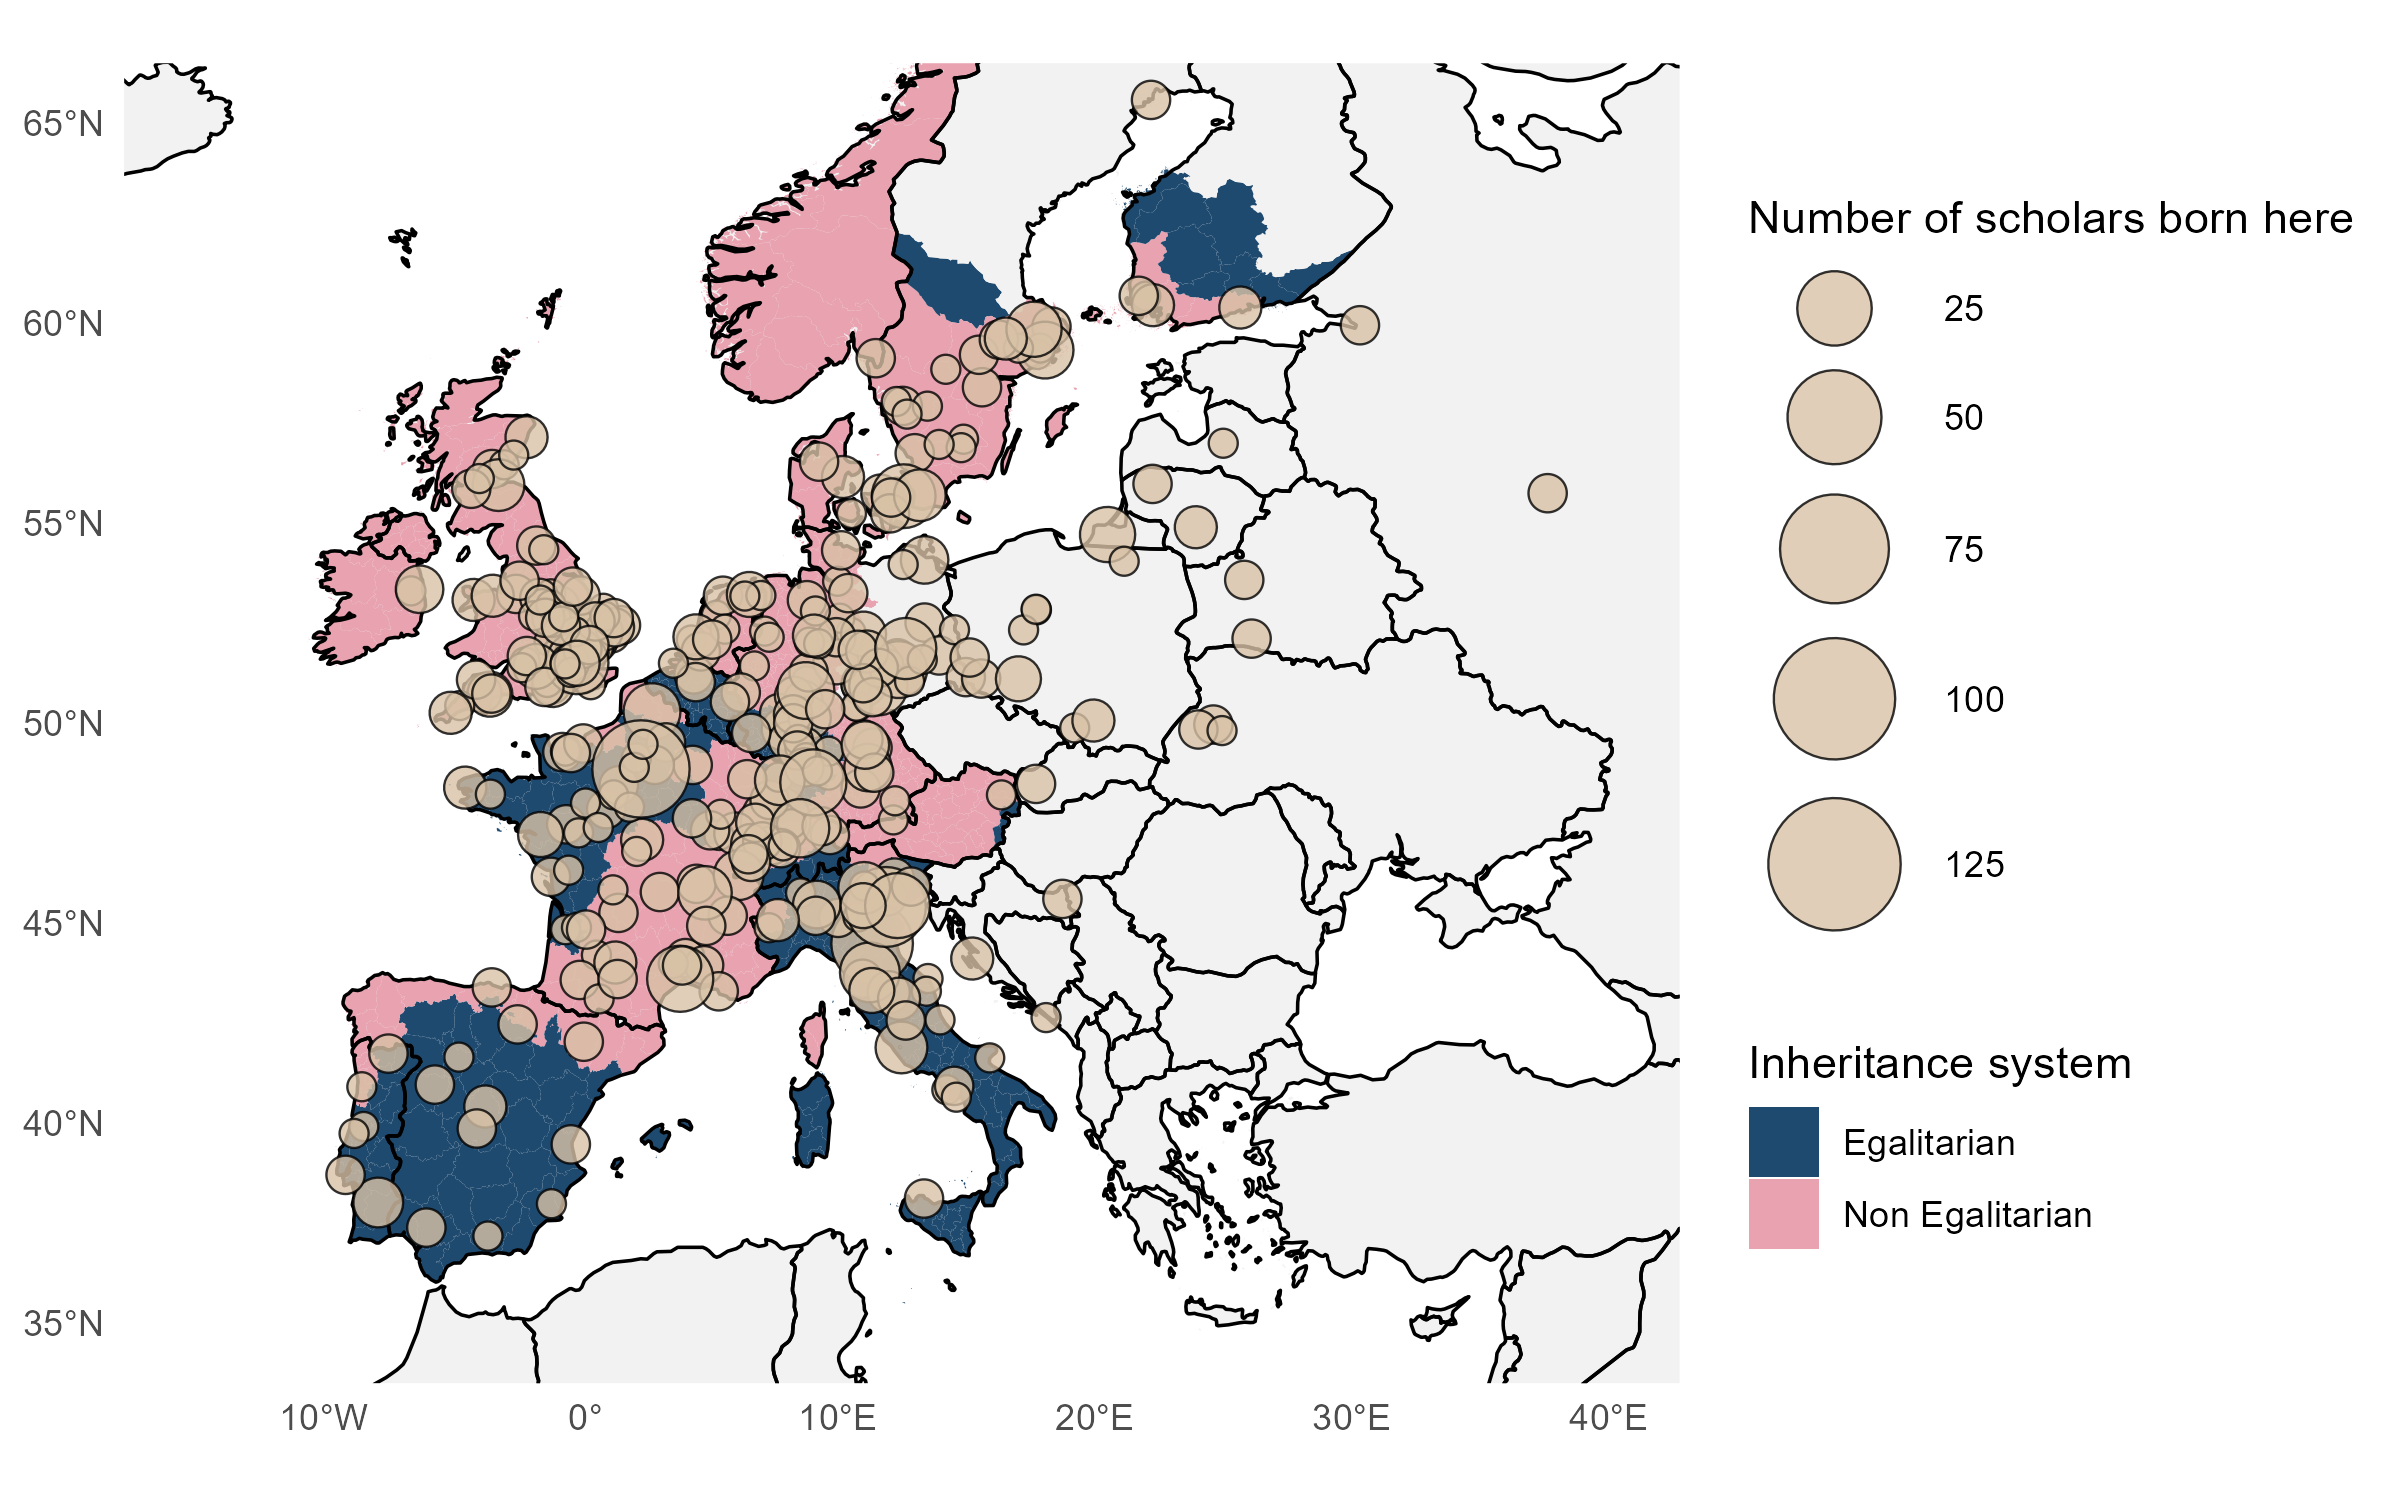
\includegraphics[width=0.85\textwidth]{figures/Map_Birthplaces_ToddColors.png}

\caption{Birthplaces of Scholars and Inheritance Systems in Europe}
\label{fig:todd_map}

\vspace{4pt}
\begin{minipage}{\textwidth}
\footnotesize
\textit{Notes:} The map displays the birthplaces of scholars belonging to the analytical sample of rankable brother pairs with identifiable birth locations, together with the classification of inheritance systems across European regions. Inheritance regimes are assigned at the NUTS3 level following Todd's classification. The figure provides a descriptive illustration of the geographical distribution of rankable scholarly brother pairs and inheritance systems across Europe. Circles indicate the number of scholars born in each location.
\end{minipage}

\end{figure}
\FloatBarrier

\begin{figure}[H]
\centering
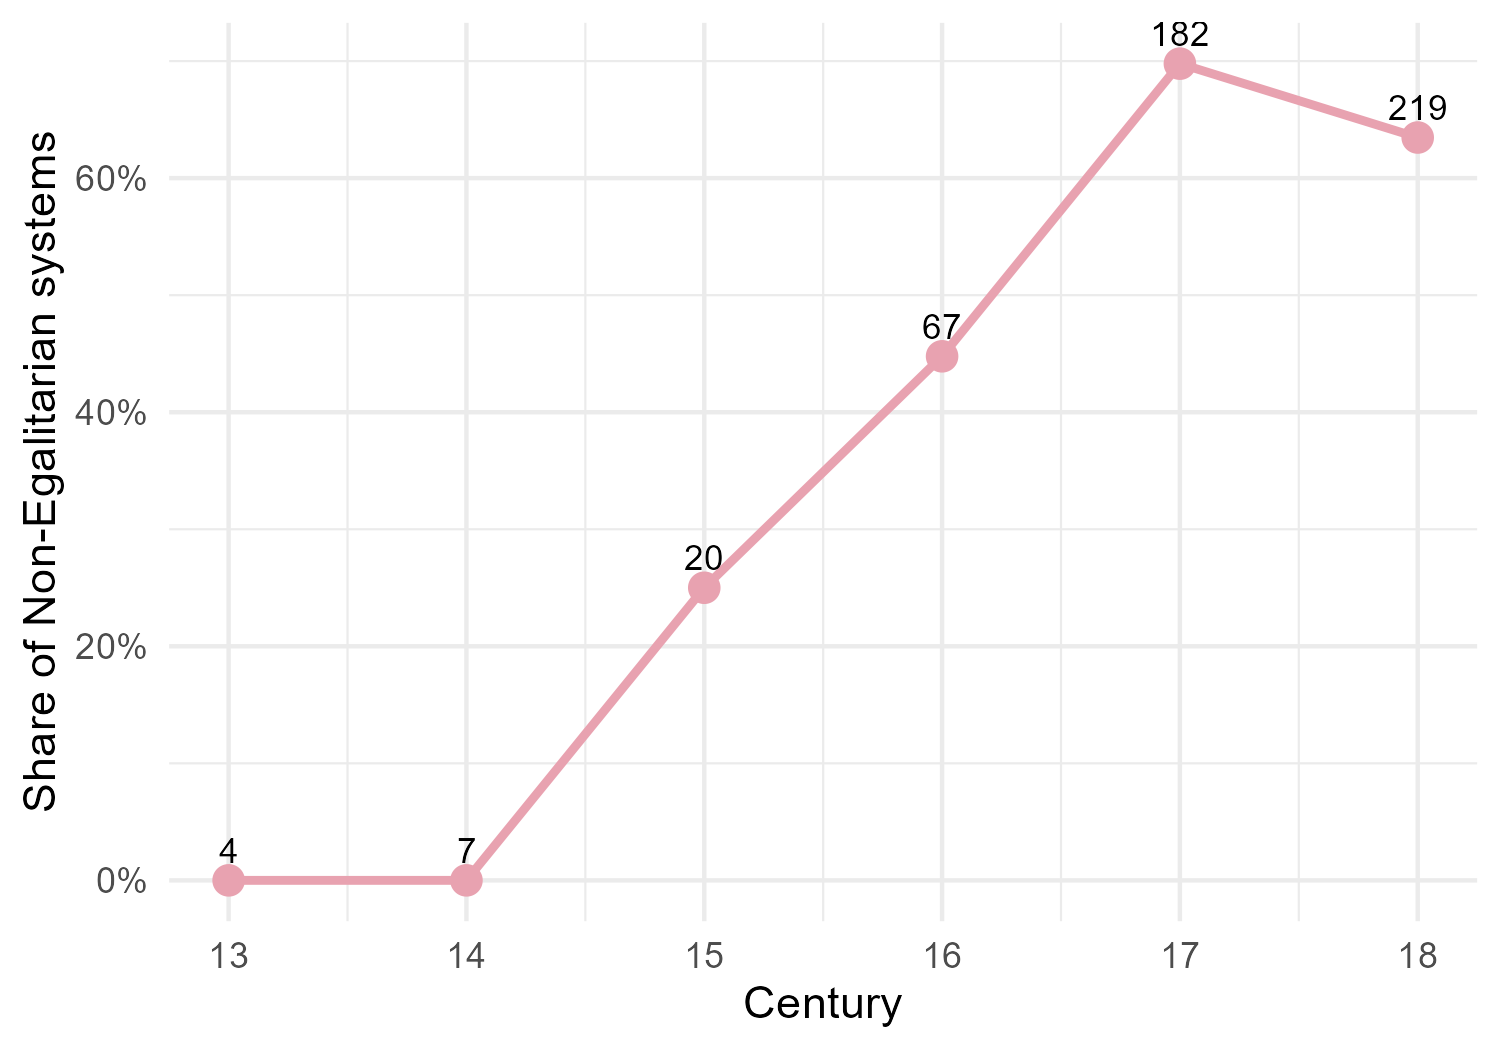
\includegraphics[width=0.65\textwidth]{figures/Inheritance_by_Century.png}

\caption{Share of Brother Pairs from Non-Egalitarian Inheritance Regions by Century}
\label{fig:inheritance_century}

\vspace{4pt}
\begin{minipage}{\textwidth}
\footnotesize
\textit{Notes:} The figure shows the share of rankable brother pairs from non-egalitarian inheritance regions by century. Inheritance regimes are assigned based on the birthplace of the older brother, following Todd's classification. Numbers above the points indicate the total number of brother pairs observed in each century.
\end{minipage}

\end{figure}
\FloatBarrier

\phantomsection
\subsection*{3.5 Regression Analysis}
\addcontentsline{toc}{subsection}{3.5 Regression Analysis}

To quantify birth-order differences in scholarly productivity, we estimate regression models where the dependent variable is the inverse hyperbolic sine transformation of the difference in title counts between older and younger brothers. Positive values indicate higher productivity for the older sibling. Because the empirical specification relies on comparisons between older and younger siblings, brother pairs with identical recorded birth years are excluded from the regression analysis.

The baseline empirical specification is estimated using ordinary least squares and can be written as:
\begin{align*}
\Delta Productivity_i
=
&\,
\beta_0
+
\beta_1 AgeGap_i
+
\beta_2 FatherAcademia_i
\\
&+
\beta_3 DifferentInstitution_i
+
\beta_4 NonEgalitarian_i
\\
&+
\beta_5 UnknownInheritance_i
+
\varepsilon_i
\end{align*}

where $\Delta Productivity_i = \operatorname{asinh}(Titles^{Older}_i) - \operatorname{asinh}(Titles^{Younger}_i)$. This specification measures within-family differences in scholarly productivity in transformed units while remaining well-defined in the presence of zero publication counts.

$AgeGap_i$ is a continuous variable measuring the age difference in years between siblings. $FatherAcademia_i$ is a binary indicator equal to one if the father was active in academia. $DifferentInstitution_i$ is a binary indicator equal to one if the two brothers are associated with different academic institutions. $NonEgalitarian_i$ and $UnknownInheritance_i$ are binary indicators capturing the inheritance regime of the birthplace region of the older brother, with egalitarian inheritance systems used as the omitted reference category. 

In this specification, $\beta_1$ captures how productivity differences vary with sibling age gaps, $\beta_2$ captures differences associated with paternal academic background, $\beta_3$ measures the association between institutional divergence and productivity gaps, while $\beta_4$ and $\beta_5$ capture differences associated with inheritance systems relative to egalitarian regions. 

The constant term therefore represents the expected productivity difference for brother pairs from egalitarian inheritance regions, sharing the same institution, without a father in academia, and with an age gap equal to zero. Since observations with exactly zero age gaps are largely absent from the sample, the constant should not be interpreted literally but rather as a baseline reference category for the regression.

The preferred specification additionally includes century indicator variables in order to account for broad historical differences in scholarly production, intellectual institutions, and the preservation of historical records across periods. The specification becomes:
\begin{align*}
\Delta Productivity_i
=
&\,
\beta_0
+
\beta_1 \textit{AgeGap}_i
+
\beta_2 \textit{FatherAcademia}_i
\\
&+
\beta_3 \textit{DifferentInstitution}_i
+
\beta_4 \textit{NonEgalitarian}_i
\\
&+
\beta_5 \textit{UnknownInheritance}_i
+
\sum_{c=13}^{17} \gamma_c Century_{ic}
+
\varepsilon_i
\end{align*}
where $Century_{ic}$ is an indicator variable equal to one if brother pair $i$ belongs to century $c$, and zero otherwise, for centuries thirteen through seventeen. The eighteenth century is used as the omitted reference category. Each $\gamma_c$ therefore captures the difference in the older-younger productivity gap relative to eighteenth-century brother pairs, holding the other covariates constant.

Table~\ref{tab:main_regressions} reports the results. Across specifications, the estimates suggest modest but persistent productivity differences favoring older brothers, although the mechanisms underlying these differences vary across historical periods. In baseline specifications, larger age gaps between siblings are associated with larger productivity differences. The positive coefficient on age differences suggests that, holding other observed characteristics constant, brother pairs with larger age gaps tend to display somewhat larger productivity differences in favor of the older sibling, although this relationship becomes statistically weaker once century indicators are introduced.

Family background does not appear to play a statistically significant equalizing role. The coefficient on father in academia is negative but not statistically significant, suggesting no robust evidence that shared access to academic networks reduces within-family productivity differences.

In contrast, differences in institutional affiliation emerge as a more robust determinant of within-family productivity differences. Brother pairs affiliated with different academic institutions tend to display larger productivity gaps across specifications, particularly after the sixteenth century. Across the main specifications, the coefficient on different institutions is 0.485. Evaluated at average productivity levels, this implies a productivity gap approximately 61.4\% larger for brother pairs affiliated with different institutions:
\[
100 \times
\left(
\frac{
\sinh\left(
\operatorname{asinh}(9.79)+0.485
\right)
}{
9.79
}
-1
\right)
\approx 61.4\%.
\]
Holding other observed characteristics constant, brother pairs affiliated with different institutions display productivity gaps approximately 61.4\% larger on average than pairs sharing the same institutional environment.

This suggests that institutional environments may play an important role in shaping divergent scholarly trajectories and that shared institutional environments may partially attenuate within-family productivity differences.

Additional regressions reported in Table~\ref{tab:period_regressions} reveal substantial heterogeneity across historical periods and suggest that productivity differences between brothers were driven by different mechanisms before and after the sixteenth century.

Before the sixteenth century, larger age gaps between siblings were robustly associated with larger productivity differences across specifications, even after controlling for century fixed effects, although this subsample remains relatively small. These early-period estimates should be interpreted cautiously. The pre-sixteenth-century subsample contains a relatively small number of observations and likely over-represents highly visible scholarly families for whom detailed historical records survive. In addition, institutional and inheritance-system variation is substantially more limited during the earlier centuries of the sample, making it more difficult to disentangle the effects of age gaps from broader historical and selection effects. One possible interpretation is that age differences reflected stronger cohort, seniority, and life-cycle advantages in medieval and early Renaissance academic environments, where access to scholarly careers remained relatively concentrated.

By contrast, after the sixteenth century, the age-gap effect becomes statistically weak, while differences in institutional affiliation emerge as a much more robust determinant of productivity divergence between brothers. This pattern is consistent with the growing differentiation and expansion of European universities and intellectual networks after the early modern period. As academic institutions became increasingly specialized and geographically dispersed, institutional environments appear to have played a more important role in shaping divergent scholarly trajectories within the same family.

Additional specifications reported in Appendix Table~\ref{tab:inheritance_post15} examine whether the relationship between inheritance systems and productivity differences changes after the sixteenth century using the full sample. The interaction terms suggest that the relationship between inheritance systems and productivity differences remains insignificant.

These findings suggest that while inheritance systems influenced family structures and economic incentives in historical Europe, their direct effect on productivity gaps was limited. Academic careers likely depended on other factors, including access to institutions and intellectual networks. This result is in line with recent evidence pointing towards a rather restricted role of family institutions for within-family inequality \citep{Gobbi2025}.

In summary, we do not find evidence that inheritance systems generally have a direct impact on within-family productivity differences. While inheritance regimes influenced family structures and economic incentives in historical Europe, the empirical results suggest that institutional environments and historical context played a more important role in explaining productivity divergence between siblings.

These results contribute to the mixed evidence in the literature. While modern studies find consistent advantages for earlier-born siblings, recent historical evidence points to smaller or less systematic effects \citep{ClarkCummins2024}. Our findings suggest that such effects may emerge more clearly within elite populations, such as scholars.

\begin{table}[H]
\centering
\caption{Determinants of the Birth-Order Productivity Gap}
\label{tab:main_regressions}

\begin{tablebody}
\begin{tabular}{l c c c c}
\toprule
 & (1) & (2) & (3) & (4)\\
 & \multicolumn{4}{c}{\textit{Asinh difference in titles}} \\
\midrule

Constant
& 0.083
& 0.023
& 0.005
& -0.162 \\
& (0.109)
& (0.126)
& (0.177)
& (0.197) \\

Age gap 
& 0.023** & 0.022** & 0.022** & 0.019* \\
& (0.010) & (0.010) & (0.010) & (0.011) \\

Father in academia 
&  & -0.184 & -0.186 & -0.163 \\
&  & (0.149) & (0.148) & (0.150) \\

Different institution 
&  & 0.440** & 0.440** & 0.485*** \\
&  & (0.181) & (0.181) & (0.180) \\

Non-egalitarian inheritance 
&  &  & 0.031 & 0.135 \\
&  &  & (0.169) & (0.175) \\

Unknown inheritance system
&  &  & 0.019 & 0.130 \\
&  &  & (0.198) & (0.205) \\

13th century
& & & & 0.099 \\
& & & & (0.223) \\

14th century
& & & & 1.764*** \\
& & & & (0.552) \\

15th century
& & & & 0.863** \\
& & & & (0.345) \\

16th century
& & & & 0.025 \\
& & & & (0.226) \\

17th century
& & & & 0.099 \\
& & & & (0.161) \\

\midrule
Century controls & No & No & No & Yes \\
Clustered SE (family) & Yes & Yes & Yes & Yes \\
\midrule
Observations & 645 & 645 & 645 & 645 \\
R$^{2}$ & 0.005 & 0.020 & 0.020 & 0.035 \\
Adj. R$^{2}$ & 0.004 & 0.015 & 0.012 & 0.020 \\
\bottomrule
\end{tabular}
\end{tablebody}

\vspace{4pt}
\begin{minipage}{\textwidth}
\footnotesize
\textit{Notes:} The dependent variable is the inverse hyperbolic sine (asinh) difference in titles between older and younger brothers. Positive values indicate higher productivity for the older sibling. Standard errors clustered at the family level are reported in parentheses. Column (4) includes century indicator variables, with the 18th century used as the omitted reference category.

\textit{Significance levels:} *** $p<0.01$, ** $p<0.05$, * $p<0.10$.
\end{minipage}

\end{table}
\FloatBarrier

\begin{table}[H]
\centering
\caption{Birth-Order Productivity Differences Across Historical Periods}
\label{tab:period_regressions}

\begin{tablebody}
\begin{tabular}{l c c}
\toprule
 & (1) & (2) \\
 & \textit{Before 16th century} & \textit{16th century onward} \\
\midrule
 & \multicolumn{2}{c}{\textit{Asinh difference in titles}} \\
\midrule

Constant
& -0.207 & -0.147 \\
& (0.689) & (0.200) \\

Non-egalitarian inheritance
& -0.719 & 0.164 \\
& (0.584) & (0.180) \\

Inheritance unknown
& -1.730 & 0.175 \\
& (1.724) & (0.207) \\

Age gap
& 0.110*** & 0.013 \\
& (0.031) & (0.011) \\

Father in academia
& 0.415 & -0.160 \\
& (0.771) & (0.154) \\

Different institution
& 0.995 & 0.474** \\
& (0.643) & (0.184) \\

Century 13
& -1.595*** & --- \\
& (0.584) & --- \\

Century 14
& 1.202 & --- \\
& (0.744) & --- \\

Century 16
& --- & 0.032 \\
& --- & (0.226) \\

Century 17
& --- & 0.102 \\
& --- & (0.161) \\

\midrule
Century controls & Yes & Yes \\
Clustered SE (family) & Yes & Yes \\
\midrule
Observations & 33 & 612 \\
R$^{2}$ & 0.387 & 0.020 \\
Adj. R$^{2}$ & 0.215 & 0.008 \\
\bottomrule
\end{tabular}
\end{tablebody}

\vspace{4pt}
\begin{minipage}{\textwidth}
\footnotesize
\textit{Notes:} The dependent variable is the inverse hyperbolic sine (asinh) of the difference in titles between older and younger brothers. Column (1) reports estimates for scholars born before the sixteenth century, while Column (2) reports estimates for scholars born from the sixteenth century onward. All specifications include century controls. The omitted century category is the 15th century in Column (1) and the 18th century in Column (2). Standard errors clustered at the family level are reported in parentheses.

\textit{Significance levels:} *** $p<0.01$, ** $p<0.05$, * $p<0.10$.
\end{minipage}

\end{table}
\FloatBarrier

\phantomsection
\subsection*{3.6 Robustness and Final Interpretation}
\addcontentsline{toc}{subsection}{3.6 Robustness and Final Interpretation}

Several different specifications and sample restrictions are applied in order to test the robustness of the birth-order results.

First, we limit the sample to brother pairs with an age difference of no more than twenty years (Appendix Table~\ref{tab:robustness}, Column 1). This addresses the concern that very large age differences between siblings may have more to do with differences in generational context than actual sibling comparisons. The estimated coefficients remain broadly similar in magnitude to the baseline results, implying that the primary findings are usually not driven by excessive age variations. 

Second, we limit the sample to families with two sons (Appendix Table~\ref{tab:robustness}, Column 2). This specification removes cases in which larger families generate multiple brother pairs and therefore focuses on simpler sibling structures.  Despite the smaller sample size, the estimated coefficients remain broadly consistent with the baseline specification.

Third, we repeat the analysis with alternative measures of scholarly visibility (Appendix Table~\ref{tab:alt_measures}). Furthermore, we look at the length of the scholar's Wikipedia page, the number of language versions that exist on Wikipedia, and the number of publishers associated with their works. These variables capture broader dimensions of scholarly visibility and intellectual prominence beyond publication counts. 

Fourth, we replicate the main specifications using alternative functional forms for productivity differences. In addition to the baseline inverse hyperbolic sine transformation, the regressions are re-estimated using logarithmic and level specifications of title differences (Appendix Tables~\ref{tab:log_regressions} and~\ref{tab:levels_regressions}). The logarithmic specification is implemented as $\log(x + \varepsilon)$ with $\varepsilon = 0.1$ in order to accommodate zero observations while minimizing distortions for positive productivity values close to zero.

The results obtained using the logarithmic specification are quantitatively very similar to those based on the inverse hyperbolic sine transformation. In the preferred logarithmic specification, the coefficient on different institutions is approximately 0.58. Under the logarithmic specification, percentage differences are interpreted using: $100 \times \left(e^{\beta}-1\right)$. Applying this transformation gives: $100 \times \left(e^{0.58}-1\right) \approx 78.6\%$.

In the preferred logarithmic specification, holding other observed characteristics constant, brother pairs affiliated with different institutions display productivity gaps approximately 78.6\% larger on average than pairs sharing the same institutional environment.

Although this interpretation depends on the choice of the adjustment parameter $\varepsilon$ used to accommodate zero observations, the estimated magnitudes remain broadly consistent with the baseline asinh and level specifications.

In particular, the positive association between differences in institutional affiliation and productivity divergence between siblings remains stable across specifications, suggesting that the main findings are not driven by the specific treatment of highly skewed productivity measures.

The level specifications lead to the same qualitative conclusions. In these regressions, coefficients are interpreted directly in terms of differences in the number of recorded titles between older and younger brothers. For example, the coefficient on different institutions in the preferred specification implies that, holding other observed characteristics constant, brother pairs affiliated with different institutions display productivity gaps approximately five titles larger on average. Although the level specification is more sensitive to extreme observations due to the highly skewed distribution of scholarly output, the overall pattern of results remains consistent with the baseline asinh specifications.

The magnitude of the estimates is also broadly comparable across functional forms. Evaluated at the mean productivity level of younger brothers ($y_0 = 9.79$ titles), the preferred asinh specification implies a productivity gap of approximately 61\%, corresponding to roughly six additional recorded titles at the mean productivity level. This magnitude is close to the estimates obtained in the level specifications, reinforcing the overall consistency of the results across alternative specifications.

Additional period-specific specifications for the logarithmic and level regressions are reported in Appendix Tables~\ref{tab:period_log_appendix} and~\ref{tab:period_levels_appendix}. These regressions estimate the models separately before and after the sixteenth century in order to evaluate whether the historical heterogeneity identified in the baseline specifications remains robust across alternative functional forms.

The period-specific logarithmic specifications remain closely aligned with the baseline findings. Before the sixteenth century, larger age gaps between siblings remained strongly associated with larger productivity differences, even after controlling for century fixed effects, whereas after the sixteenth century, differences in institutional affiliation emerged as the more robust correlate of within-family productivity divergence.

Some differences nevertheless emerge in the pre-sixteenth-century level specifications. In these regressions, non-egalitarian inheritance systems and differences in institutional affiliation become statistically significant, while the age-gap effect remains positive and statistically significant. Given the small size of the early-period subsample and the sensitivity of level specifications to extreme observations, these estimates likely reflect the influence of a limited number of highly productive scholarly families and the greater impact of outliers in untransformed productivity measures.

%Finally, Appendix Table~\ref{tab:region_fe_appendix} introduces additional regional controls at the NUTS level in order to account for persistent regional differences in institutional environments, economic conditions, and historical academic traditions. Regions with fewer than 10 observations are grouped into an ``Other'' category, and the most represented region in the sample is used as the reference category. Once these regional controls are included, the estimated coefficients lose statistical significance, although their signs remain broadly consistent with the baseline specifications. One important limitation is that the regional distribution of observations remains highly fragmented. Even the largest individual region contains only 33 observations, while most regions include between 10 and 20 observations. This substantially reduces statistical precision and makes it difficult to identify robust within-region patterns. 

Finally, Appendix Table~\ref{tab:country_fe_appendix} introduces additional country controls in order to account for persistent cross-country differences in institutional environments, economic conditions, and historical academic traditions. The distribution of observations across countries is highly uneven, with a small number of countries accounting for most of the sample. Germany contains 116 observations, followed by the United Kingdom (111), France (104), and Italy (96), while several remaining countries contain only a limited number of observations. Once country controls are included, the main coefficients remain broadly consistent with the baseline specifications, although some estimates become less precisely estimated. Overall, the results suggest that the observed productivity differences are not solely driven by broad country-level heterogeneity, while also indicating that part of the variation may reflect wider national institutional and academic environments.

The robustness exercises considered together suggest that the main findings are not coming from specific sample choices or from the particular measure of scholarly productivity employed. Though the magnitude of the coefficients differs between specifications, the overall pattern remains broadly consistent with a modest birth-order effect in scholarly productivity, although the estimated magnitudes vary across historical periods and empirical specifications.

Overall, the results provide evidence of a modest birth-order effect in scholarly productivity among historical European scholars. This effect appears to operate primarily through differences in access to scholarly activity rather than through conditional productivity differences among active scholars. The broad consistency of the results across inverse hyperbolic sine, logarithmic, and level specifications further suggests that the main conclusions are not driven by the particular transformation used to measure scholarly productivity.

The findings also indicate substantial historical heterogeneity. Before the sixteenth century, productivity differences between brothers appear more closely associated with sibling age gaps, whereas after the sixteenth century, institutional divergence becomes more strongly associated with within-family productivity differences. This suggests that the increasing differentiation of European academic institutions may have amplified divergent scholarly trajectories within the same family.

The results suggest that institutional environments are more consistently associated with productivity differences than inheritance systems.